\documentclass[10pt]{article}

\usepackage[margin=0.68in]{geometry}
\usepackage{amsmath,amssymb}
\usepackage{booktabs}
\usepackage{caption}
\usepackage{enumitem}
\usepackage{float}
\usepackage{graphicx}
\usepackage{microtype}
\usepackage[hidelinks]{hyperref}

\graphicspath{{../assets/figures/}}
\newcommand{\SampleObjectiveValue}{0.04597}


\setlength{\parindent}{0pt}
\setlength{\parskip}{3pt}
\setlist[itemize]{leftmargin=*,topsep=2pt,itemsep=1pt,parsep=0pt}
\setlist[enumerate]{leftmargin=*,topsep=2pt,itemsep=1pt,parsep=0pt}
\captionsetup{font=small,skip=3pt}

\title{Counterfactual Analysis for Structural Dynamic Discrete Choice Models}
\author{Kosuke Shimamoto}
\date{}

\begin{document}

\maketitle
\vspace{-2.2em}

\section{Goal}

\begin{itemize}
    \item Build validated replication code for a dynamic discrete-choice model with partially identified payoffs.
    \item Compare entry-cost and marginal-cost subsidies while carrying payoff uncertainty into every counterfactual outcome.
\end{itemize}

\section{Setting and Data-Generating Process}

\subsection{Model setup}

\begin{itemize}
    \item A single firm chooses whether to be inactive, $a_t=0$, or active, $a_t=1$.
    \item The state is $x_t=(k_t,w_t)$, where $k_t=a_{t-1}\in\{0,1\}$ and the observed profit state is $w_t\in\{L,H\}$.
    \item The profit state follows a known transition matrix $P$, independently of the current action, and $k_{t+1}=a_t$.
    \item The model has state-specific scrap values $s_w$, entry costs $e_w$, and running costs $r_w$. Entry and running costs are nonnegative.
\end{itemize}

\begin{table}[H]
    \centering
    \caption{Deterministic flow payoffs}
    \begin{tabular}{ccc}
        \toprule
        Previous action & Inactive, $a_t=0$ & Active, $a_t=1$ \\
        \midrule
        $k_t=0$ & $0$ & $\pi_w-r_w-e_w$ \\
        $k_t=1$ & $s_w$ & $\pi_w-r_w$ \\
        \bottomrule
    \end{tabular}
\end{table}

The calibration uses $\pi=(2,4)$, $\beta=0.9$, a persistent two-state profit process, and true values $s=(4.5,4.5)$, $e=(5,5)$, and $r=(0.5,0.5)$. Type-I extreme-value shocks generate logit conditional choice probabilities (CCPs).

\subsection{Model solution}

Let $V(k,w)$ denote the ex-ante value. The choice-specific values satisfy

\begin{equation*}
v_a(k,w)=u(k,w,a)+\beta E[V(a,w')\mid w].
\end{equation*}

The extreme-value shocks imply the inclusive-value equation

\begin{equation*}
V(k,w)=\log\!\left(\exp(v_0(k,w))+\exp(v_1(k,w))\right),
\end{equation*}

and the active-choice probability is

\begin{equation*}
p_{kw}=\frac{\exp(v_1(k,w))}
{\exp(v_0(k,w))+\exp(v_1(k,w))}.
\end{equation*}

Value iteration solves this four-state fixed point and returns the four population CCPs.

\section{Identification}

Let $p_{kw}=\Pr(a=1\mid k,w)$ and $d_{kw}=\log[p_{kw}/(1-p_{kw})]$. For a fixed profit state, the continuation term is common across the two lagged-action states:

\begin{equation*}
C_w=\beta\sum_{w'}P_{ww'}[V(1,w')-V(0,w')].
\end{equation*}

The two log-odds equations are

\begin{equation*}
d_{0w}=\pi_w-r_w-e_w+C_w,
\qquad
d_{1w}=\pi_w-r_w-s_w+C_w.
\end{equation*}

Taking their difference eliminates the common continuation value and gives the first identifying equation:

\begin{equation*}
d_{1w}-d_{0w}=e_w-s_w.
\end{equation*}

For the second equation, compare the inactive paths $(0,w)\rightarrow(0,w')$ and $(1,w)\rightarrow(0,w')$. Their continuation values coincide. The logit inclusive-value identity therefore gives

\begin{equation*}
V(1,w)-V(0,w)
=s_w+\log\!\left(\frac{1-p_{0w}}{1-p_{1w}}\right)
=s_w+A_w(p),
\end{equation*}

where $A_w(p)=\log[(1-p_{0w})/(1-p_{1w})]$. For each candidate $s=(s_L,s_H)$, the two equations recover

\begin{equation*}
e_w(s;p)=s_w+d_{1w}-d_{0w},
\end{equation*}

\begin{equation*}
r_w(s;p)=\pi_w-e_w(s;p)
+\beta\sum_{w'}P_{ww'}[s_{w'}+A_{w'}(p)]-d_{0w}.
\end{equation*}

Nonnegative entry and running costs restrict the free scrap values to

\begin{equation*}
\mathcal S(p)=\{s\in\mathbb R^2:e_w(s;p)\geq0,\ r_w(s;p)\geq0,
\ w\in\{L,H\}\}.
\end{equation*}

The payoff identified set is

\begin{equation*}
\Theta_I(p)=\{(s,e(s;p),r(s;p)):s\in\mathcal S(p)\}.
\end{equation*}

\begin{figure}[H]
    \centering
    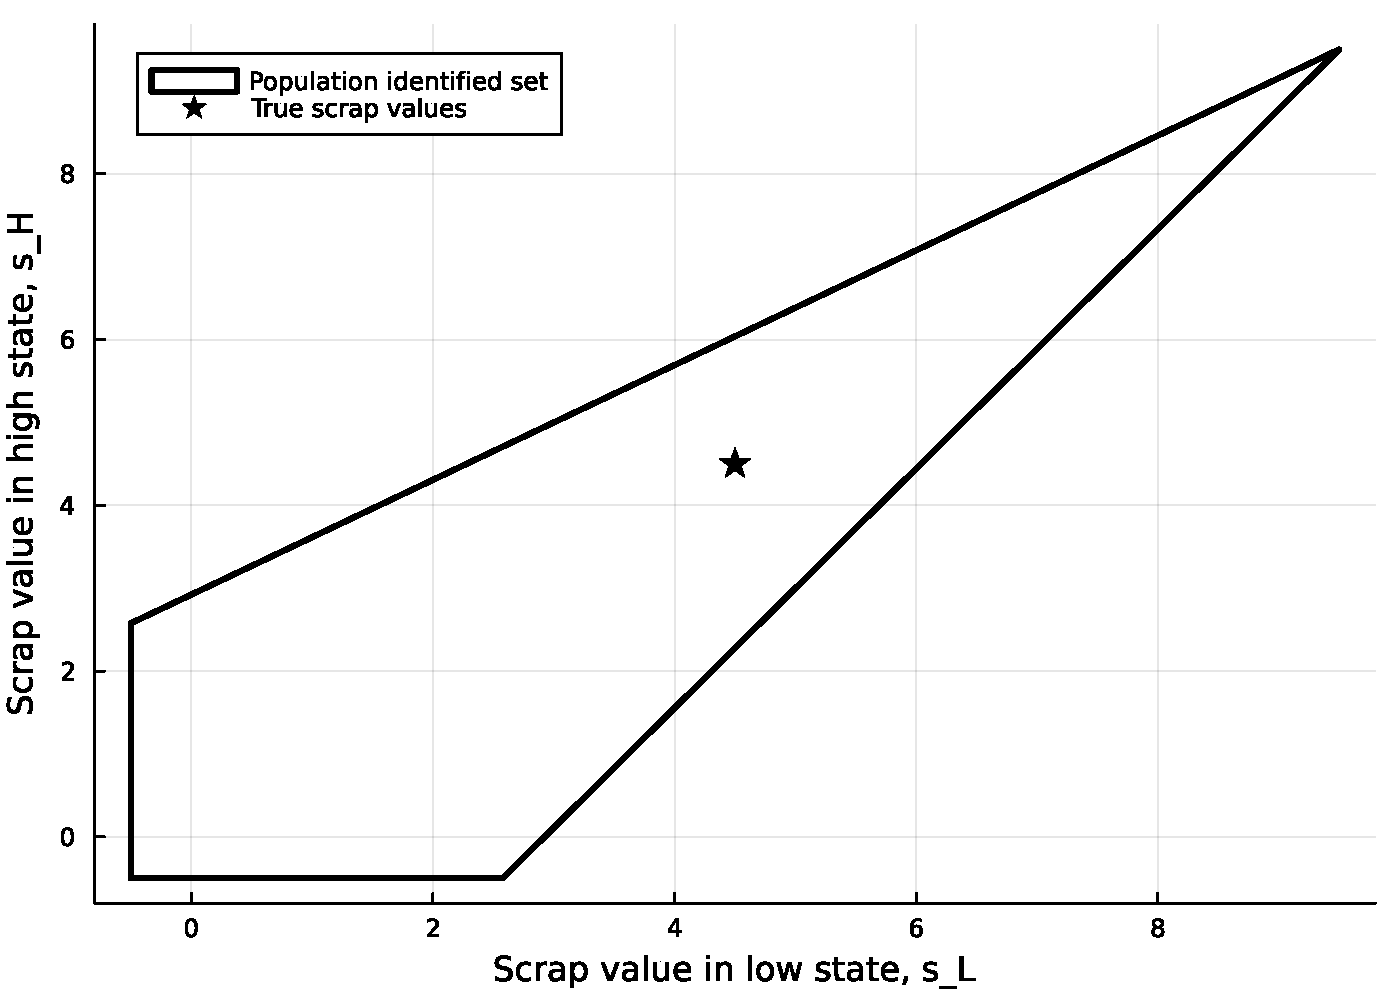
\includegraphics[width=0.52\textwidth]{population_identified_set.pdf}
    \caption{The population restrictions form a polygon in $(s_L,s_H)$. The star is the true payoff vector, which lies inside the set but is not point identified.}
\end{figure}

\section{Estimation}

\subsection{Data-generating process}

The simulation draws actions from the four population CCPs, sets $k_{t+1}=a_t$, and draws $w_{t+1}$ from $P(\cdot\mid w_t)$. The sample contains 2,000 firms observed for 20 periods.

\subsection{Summary Statistics}

\begin{table}[H]
    \centering
    \caption{State-level observations and active choices}
    \input{../assets/tables/summary_statistics.tex}
\end{table}

\subsection{Estimated CCPs}

Each CCP is the active-choice frequency in state $(k,w)$:

\begin{equation*}
\widehat p_{kw}
=\frac{\sum_{i,t}\mathbf 1\{k_{it}=k,w_{it}=w,a_{it}=1\}}
{\sum_{i,t}\mathbf 1\{k_{it}=k,w_{it}=w\}}.
\end{equation*}

\begin{table}[H]
    \centering
    \caption{Estimated and population CCPs}
    \begin{tabular}{ccrr}
\toprule
$k_t$ & Profit state & $\widehat p_{kw}$ & $p_{kw}$ \\
\midrule
0 & Low & 0.715 & 0.714 \\
0 & High & 0.956 & 0.951 \\
1 & Low & 0.801 & 0.805 \\
1 & High & 0.97 & 0.97 \\
\bottomrule
\end{tabular}

\end{table}

\subsection{Sample objective}

Replacing $p$ and $P$ with $\widehat p$ and $\widehat P$ gives four sample restrictions $\widehat m(\theta)$. With $W=I_4$, the minimum-distance objective is

\begin{equation*}
\widehat Q(\theta)=\widehat m(\theta)'\widehat m(\theta),
\qquad
\theta=(s_L,s_H,e_L,e_H,r_L,r_H).
\end{equation*}

At the true payoff vector, the sample objective equals $\SampleObjectiveValue$; sampling error prevents it from being exactly zero.

\subsection{Estimated identified set}

Plugging $\widehat p$ and $\widehat P$ into the analytic formulas for $e(s)$ and $r(s)$ yields the estimated polygon $\widehat{\mathcal S}$. A grid search checks its two-dimensional projection.

\begin{figure}[H]
    \centering
    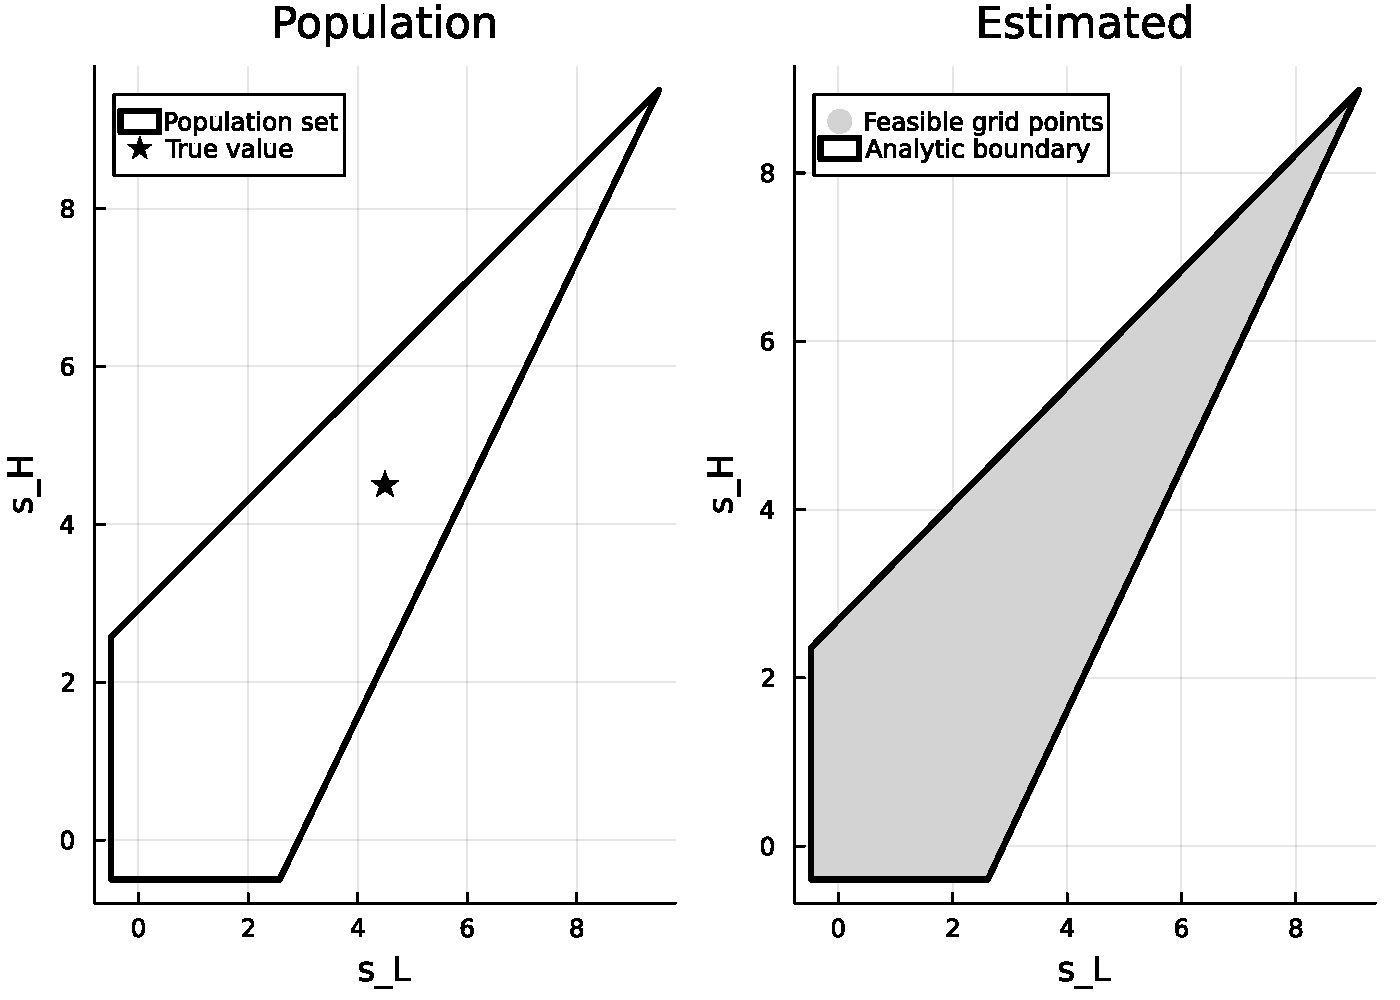
\includegraphics[width=0.86\textwidth]{estimated_identified_set.pdf}
    \caption{The population and estimated payoff sets. Gray grid points numerically reproduce the analytic estimated boundary.}
\end{figure}

\section{Counterfactual Analysis}

\subsection{Overview}

\begin{itemize}
    \item The policy grid uses $\tau_E,\tau_M\in[0,0.5]$. Entry subsidies are paid when an inactive firm enters; marginal-cost subsidies are paid whenever the firm operates.
    \item Every policy is solved for every admissible payoff vector in the estimated identified set. The minimum and maximum outcomes form numerical counterfactual bounds.
    \item The calculation covers the polygon interior, vertices, and edges. A denser grid checks the numerical approximation.
\end{itemize}

The proportional subsidies change entry and running costs to

\begin{equation*}
e_w^{cf}=(1-\tau_E)e_w,
\qquad
r_w^{cf}=(1-\tau_M)r_w.
\end{equation*}

Let $\mu_{kw}^{cf}$ denote the stationary state probability and $p_{kw}^{cf}$ the active CCP. The long-run active share and its percentage change are

\begin{equation*}
\mu_1^{cf}=\sum_{k,w}\mu_{kw}^{cf}p_{kw}^{cf},
\qquad
R_\mu=100\frac{\mu_1^{cf}-\mu_1^0}{\mu_1^0}.
\end{equation*}

Long-run expenditure per firm and period is

\begin{equation*}
G_E=\sum_w \tau_E e_w\mu_{0w}^{cf}p_{0w}^{cf},
\end{equation*}

\begin{equation*}
G_M=\sum_{k,w}\tau_M r_w\mu_{kw}^{cf}p_{kw}^{cf},
\qquad
G=G_E+G_M.
\end{equation*}

Cost-effectiveness is $CE=R_\mu/G$ when $G>0$.

\subsection{Entry Cost Subsidy}

\begin{figure}[H]
    \centering
    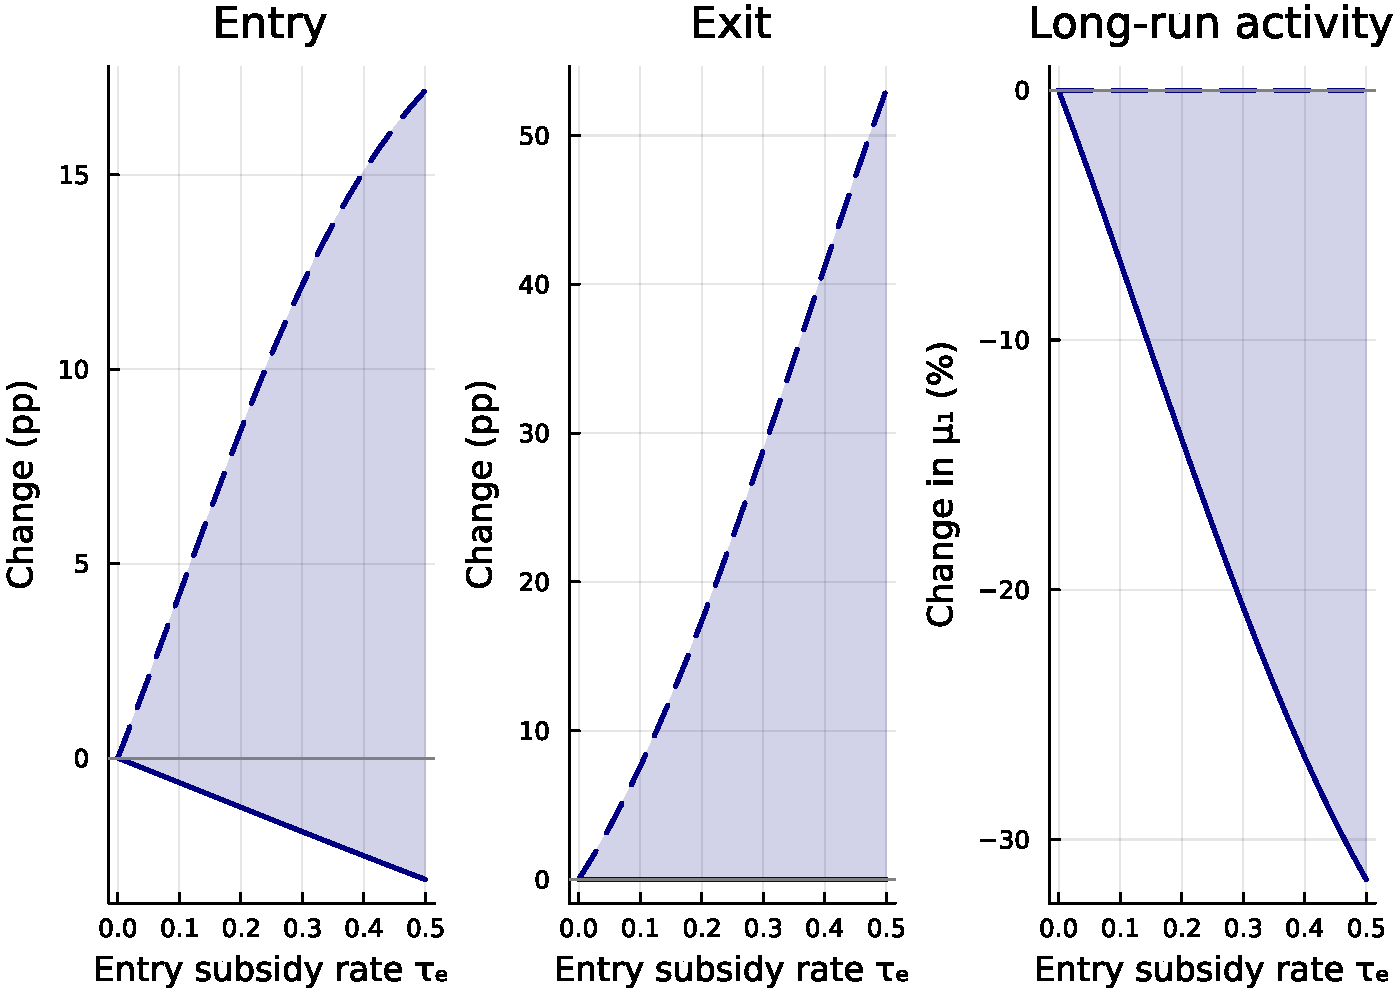
\includegraphics[width=0.95\textwidth]{entry_cost_subsidy.pdf}
    \caption{An entry-cost subsidy can increase exit as firms preserve the option to re-enter with support. Across the identified set, the exit response can dominate and reduce long-run activity.}
\end{figure}

\subsection{Marginal Cost Subsidy}

\begin{figure}[H]
    \centering
    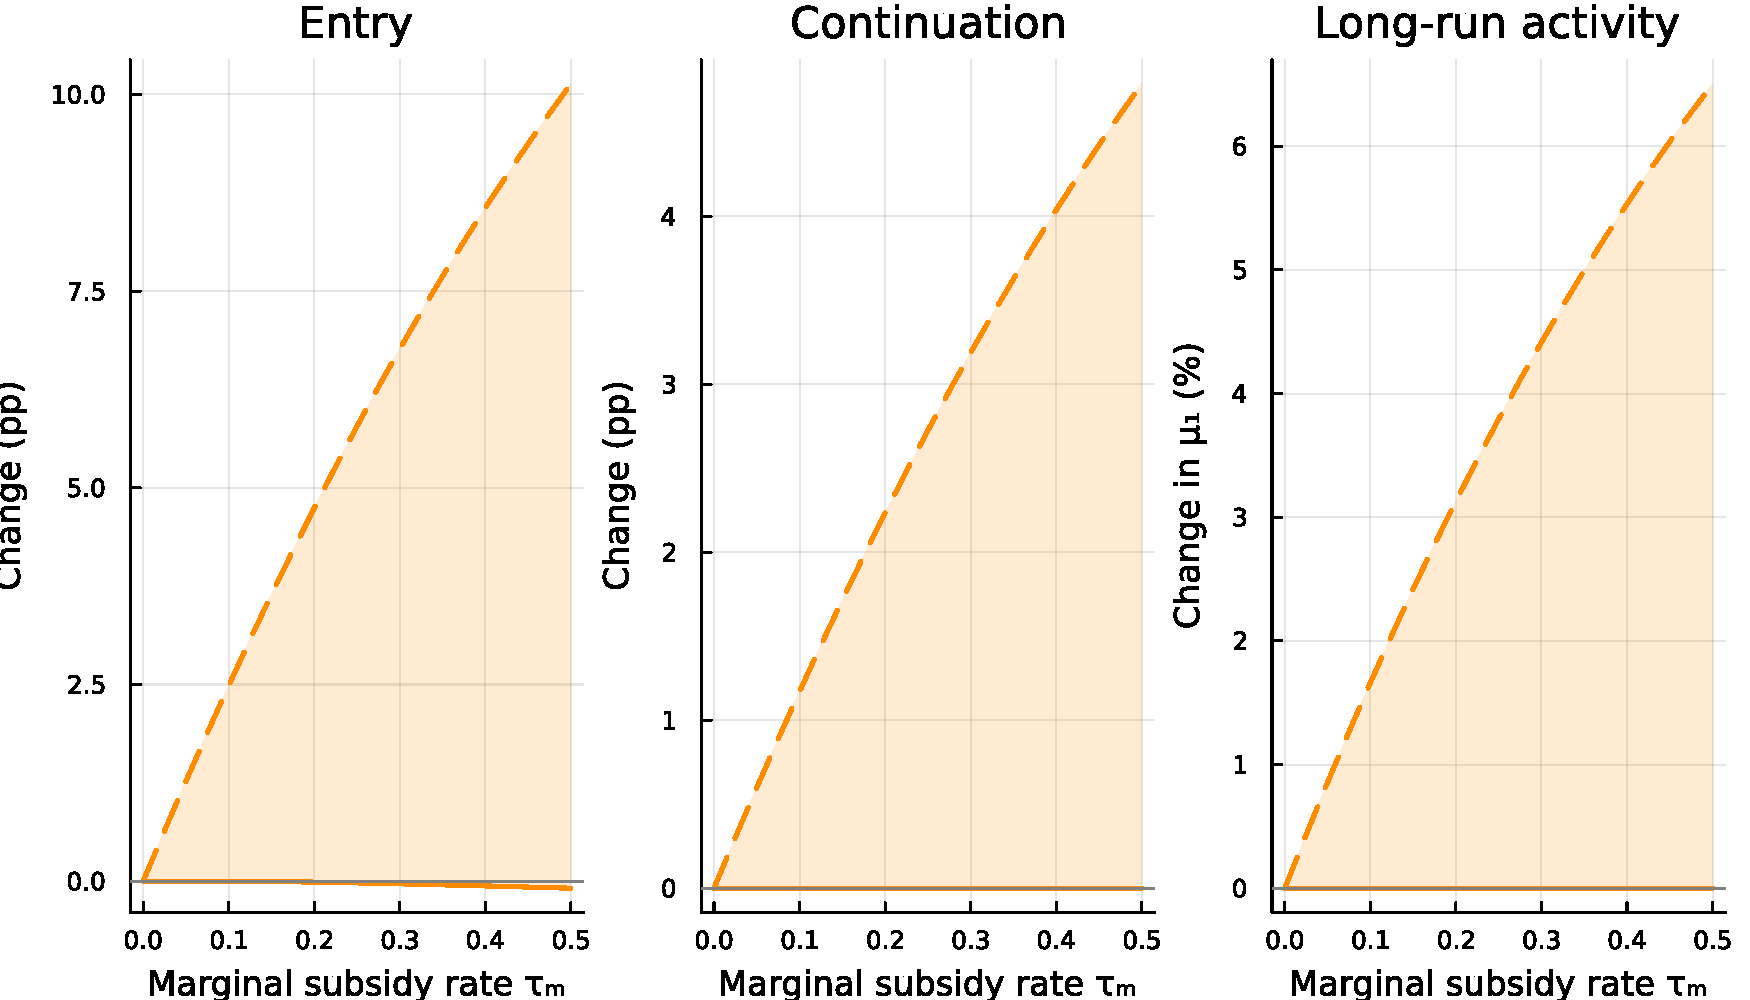
\includegraphics[width=0.95\textwidth]{marginal_cost_subsidy.pdf}
    \caption{A marginal-cost subsidy supports both entry and continued operation. The long-run active-share response is weakly positive over the estimated payoff set.}
\end{figure}

\subsection{Mixed Policy Design}

\begin{figure}[H]
    \centering
    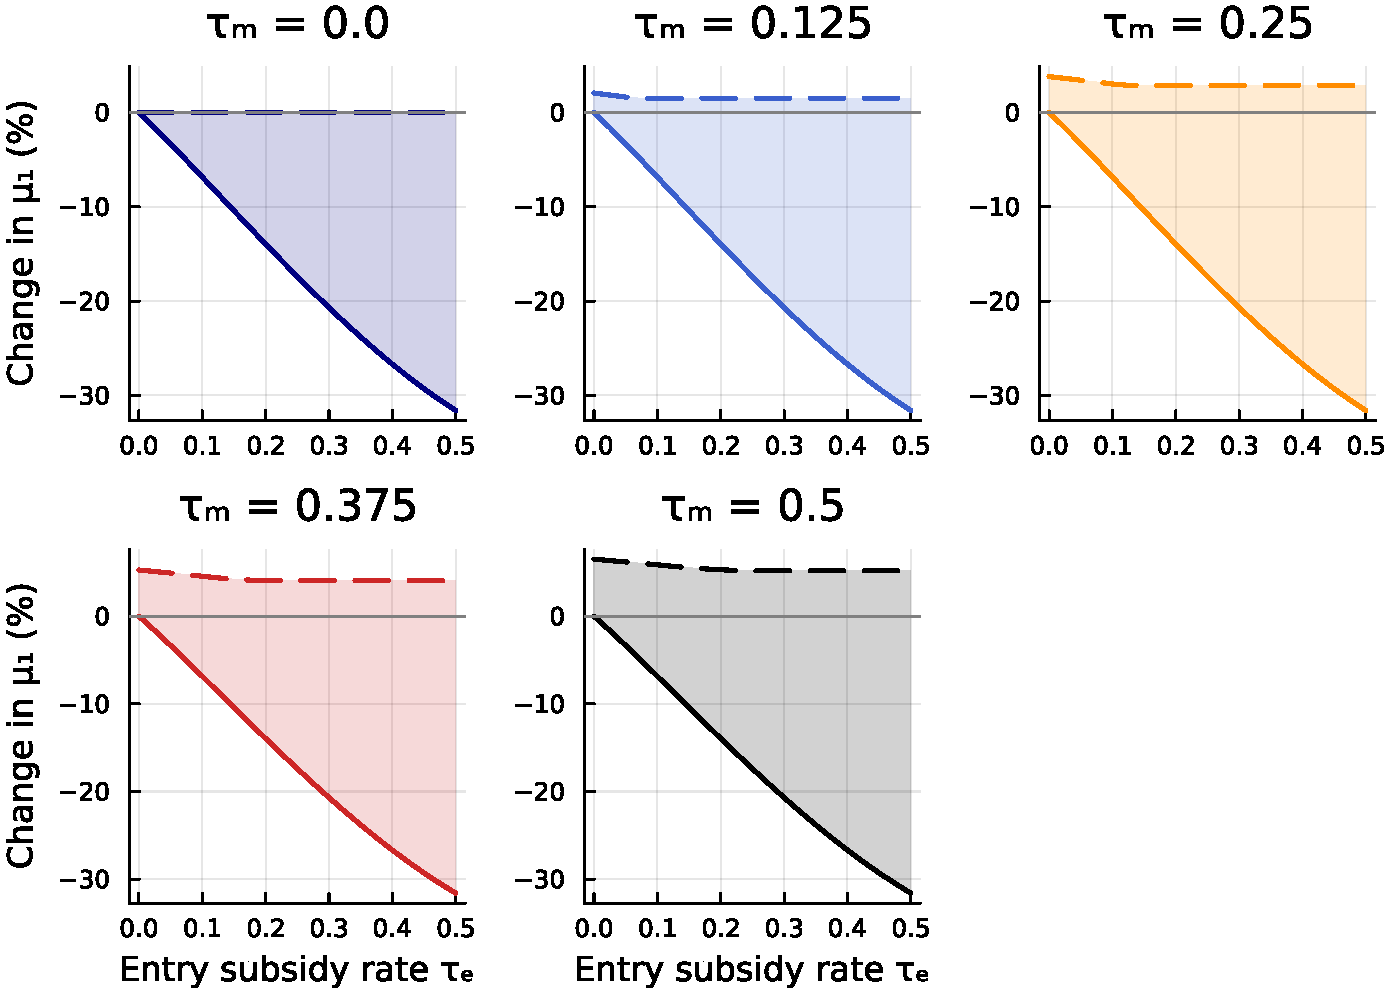
\includegraphics[width=0.90\textwidth]{mixed_active_share.pdf}
    \caption{Identified bounds for the percentage change in the stationary active share across the two-policy grid.}
\end{figure}

\begin{figure}[H]
    \centering
    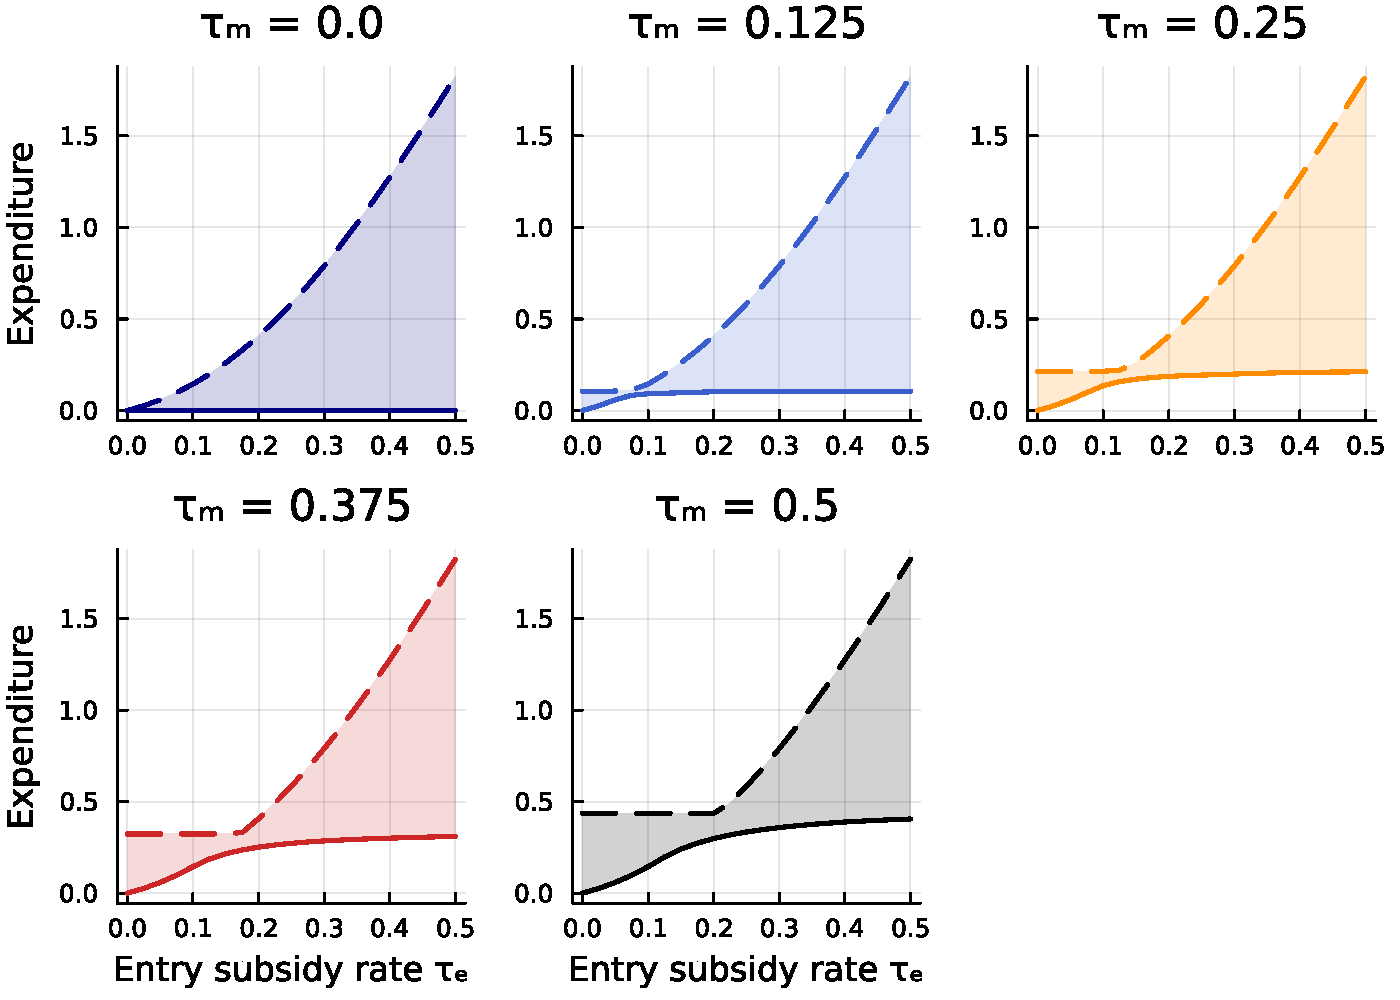
\includegraphics[width=0.90\textwidth]{mixed_expenditure.pdf}
    \caption{Identified expenditure bounds. Entry and marginal-cost subsidies differ in timing and payment frequency.}
\end{figure}

\begin{figure}[H]
    \centering
    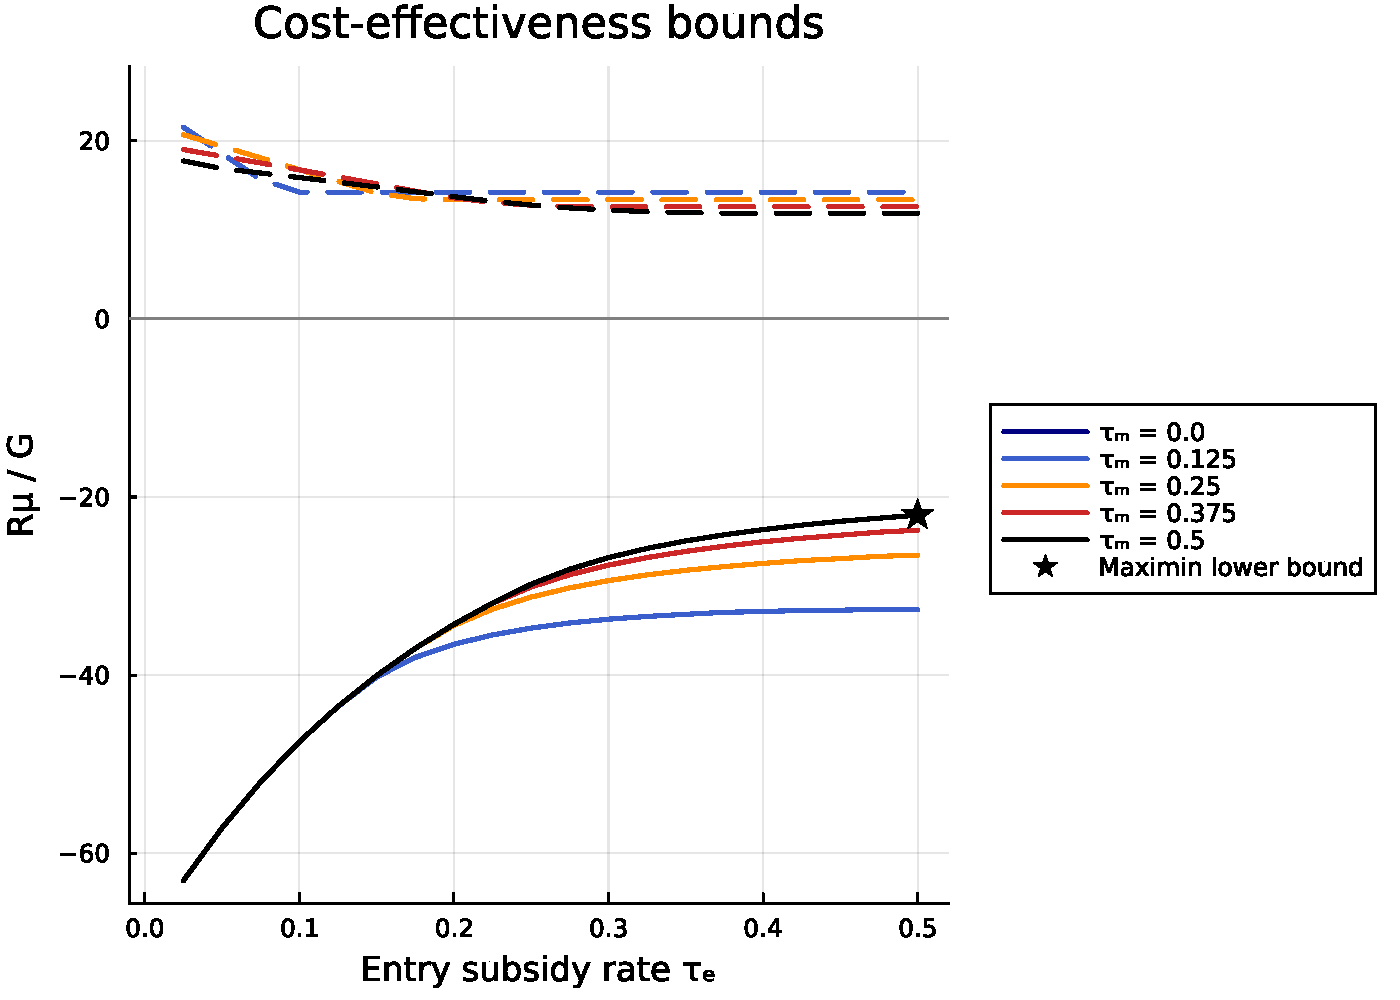
\includegraphics[width=0.72\textwidth]{mixed_cost_effectiveness.pdf}
    \caption{Lower and upper cost-effectiveness bounds. Each color fixes $\tau_M$ while $\tau_E$ varies; gaps fail the minimum-expenditure threshold.}
\end{figure}

\end{document}
